\documentclass[12pt, a4paper, twoside]{article}
\usepackage{../labreport}
\usepackage{pdfpages}

\setlabreportopts[authors={Nandor Kovacs \& Céline Schuster},
    title={Mathematisches Pendel},
    subtitle={Untersuchung der Eigenschaften eines Mathematischen Pendels},
    date={\today},
    labdate={10. März 2022}
]

\begin{document}
\maketitlepage
\includepdf[pages=2-3]{aufgabenstellung.pdf}

\section{Einleitung}
\section{Theorie}
\section{Demo 1}
\section{Demo 2}
\section{Versuch 1}
\subsection{Experimentbeschreibung}
In einer Entfernung von 20cm zum Zählrohr wird eine radioaktive Quelle platziert.
Die Schutzkappe wird von der Quelle entfernt.
Nun wird dreimal die Zeit gemessen, in der 1000 Erreignisse geschehen.
Das gleiche Experiment wird auch in einer Entfernung von 10cm ausgeführt.
\subsection{Aufgabe 1}
\subsection{Aufgabe 2}

\section{Versuch 2}
\section{Versuch 3}
\section{Fazit}
\section{Reflektion}



\end{document}
